\documentclass[11pt]{article}
\usepackage{booktabs,xcolor,pgfplots}
\pgfplotsset{compat=1.18}
\definecolor{okgreen}{RGB}{0,128,0}
\definecolor{failred}{RGB}{200,0,0}
\begin{document}
\section*{Test 2: Circle Radius and Float64 Breakdown}

\subsection*{Success by Radius}
\begin{tabular}{l|ccccccc}
\toprule
Method & $10^{-1}$ & $10^{-2}$ & $10^{-3}$ & $10^{-4}$ & $10^{-5}$ & $10^{-6}$ & $10^{-8}$ \\\midrule
BigFloat-128 & -- & -- & -- & \textcolor{okgreen}{\checkmark} & \textcolor{okgreen}{\checkmark} & \textcolor{okgreen}{\checkmark} & \textcolor{okgreen}{\checkmark} \\
BigFloat-256 & -- & -- & -- & \textcolor{okgreen}{\checkmark} & \textcolor{okgreen}{\checkmark} & \textcolor{okgreen}{\checkmark} & \textcolor{okgreen}{\checkmark} \\
Miyajima & \textcolor{okgreen}{\checkmark} & \textcolor{okgreen}{\checkmark} & \textcolor{okgreen}{\checkmark} & \textcolor{okgreen}{\checkmark} & \textcolor{okgreen}{\checkmark} & \textcolor{okgreen}{\checkmark} & \textcolor{okgreen}{\checkmark} \\
Ogita & \textcolor{okgreen}{\checkmark} & \textcolor{okgreen}{\checkmark} & \textcolor{okgreen}{\checkmark} & \textcolor{okgreen}{\checkmark} & \textcolor{okgreen}{\checkmark} & \textcolor{okgreen}{\checkmark} & \textcolor{okgreen}{\checkmark} \\
V1 & \textcolor{okgreen}{\checkmark} & \textcolor{okgreen}{\checkmark} & \textcolor{okgreen}{\checkmark} & \textcolor{okgreen}{\checkmark} & \textcolor{okgreen}{\checkmark} & \textcolor{okgreen}{\checkmark} & \textcolor{okgreen}{\checkmark} \\
V2 & \textcolor{okgreen}{\checkmark} & \textcolor{okgreen}{\checkmark} & \textcolor{okgreen}{\checkmark} & \textcolor{okgreen}{\checkmark} & \textcolor{okgreen}{\checkmark} & \textcolor{okgreen}{\checkmark} & \textcolor{okgreen}{\checkmark} \\
V2.5 & \textcolor{okgreen}{\checkmark} & \textcolor{okgreen}{\checkmark} & \textcolor{okgreen}{\checkmark} & \textcolor{okgreen}{\checkmark} & \textcolor{okgreen}{\checkmark} & \textcolor{okgreen}{\checkmark} & \textcolor{okgreen}{\checkmark} \\
V3 & \textcolor{okgreen}{\checkmark} & \textcolor{okgreen}{\checkmark} & \textcolor{okgreen}{\checkmark} & \textcolor{okgreen}{\checkmark} & \textcolor{okgreen}{\checkmark} & \textcolor{okgreen}{\checkmark} & \textcolor{okgreen}{\checkmark} \\
\bottomrule\end{tabular}

\subsection*{Breakdown Radii}
\begin{tabular}{lr}
\toprule
Method & Smallest Successful Radius \\\midrule
V3 & $1e-08$ \\
BigFloat-256 & $1e-08$ \\
V2 & $1e-08$ \\
V2.5 & $1e-08$ \\
BigFloat-128 & $1e-08$ \\
Ogita & $1e-08$ \\
Miyajima & $1e-08$ \\
V1 & $1e-08$ \\
\bottomrule\end{tabular}

\subsection*{Bound Quality vs Radius}
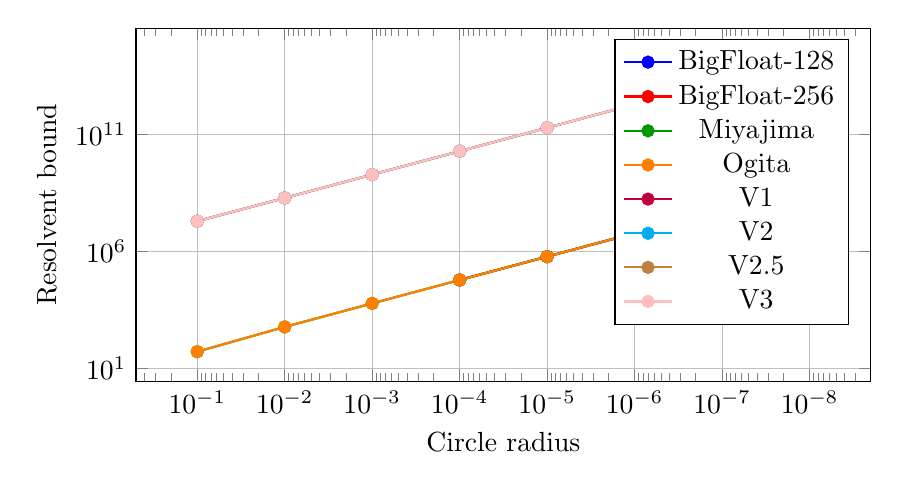
\begin{tikzpicture}
\begin{loglogaxis}[
    xlabel={Circle radius},
    ylabel={Resolvent bound},
    legend pos=north east,
    width=0.9\textwidth,
    height=0.5\textwidth,
    grid=major,
    x dir=reverse,
]

\addplot[blue, mark=*, thick] coordinates {(1.00e-04, 6.1095e+04) (1.00e-05, 6.1103e+05) (1.00e-06, 6.1104e+06) (1.00e-08, 6.1104e+08) };
\addlegendentry{BigFloat-128}
\addplot[red, mark=*, thick] coordinates {(1.00e-04, 6.1095e+04) (1.00e-05, 6.1103e+05) (1.00e-06, 6.1104e+06) (1.00e-08, 6.1104e+08) };
\addlegendentry{BigFloat-256}
\addplot[green!60!black, mark=*, thick] coordinates {(1.00e-01, 5.2768e+01) (1.00e-02, 6.0176e+02) (1.00e-03, 6.1010e+03) (1.00e-04, 6.1095e+04) (1.00e-05, 6.1103e+05) (1.00e-06, 6.1104e+06) (1.00e-08, 6.1138e+08) };
\addlegendentry{Miyajima}
\addplot[orange, mark=*, thick] coordinates {(1.00e-01, 5.2768e+01) (1.00e-02, 6.0176e+02) (1.00e-03, 6.1010e+03) (1.00e-04, 6.1095e+04) (1.00e-05, 6.1103e+05) (1.00e-06, 6.1104e+06) (1.00e-08, 6.1104e+08) };
\addlegendentry{Ogita}
\addplot[purple, mark=*, thick] coordinates {(1.00e-01, 2.0000e+07) (1.00e-02, 1.9628e+08) (1.00e-03, 1.9600e+09) (1.00e-04, 1.9598e+10) (1.00e-05, 1.9597e+11) (1.00e-06, 1.9597e+12) (1.00e-08, 1.9598e+14) };
\addlegendentry{V1}
\addplot[cyan, mark=*, thick] coordinates {(1.00e-01, 2.0000e+07) (1.00e-02, 1.9628e+08) (1.00e-03, 1.9600e+09) (1.00e-04, 1.9598e+10) (1.00e-05, 1.9597e+11) (1.00e-06, 1.9597e+12) (1.00e-08, 1.9598e+14) };
\addlegendentry{V2}
\addplot[brown, mark=*, thick] coordinates {(1.00e-01, 2.0000e+07) (1.00e-02, 1.9628e+08) (1.00e-03, 1.9600e+09) (1.00e-04, 1.9598e+10) (1.00e-05, 1.9597e+11) (1.00e-06, 1.9597e+12) (1.00e-08, 1.9598e+14) };
\addlegendentry{V2.5}
\addplot[pink, mark=*, thick] coordinates {(1.00e-01, 2.0000e+07) (1.00e-02, 1.9628e+08) (1.00e-03, 1.9600e+09) (1.00e-04, 1.9598e+10) (1.00e-05, 1.9597e+11) (1.00e-06, 1.9597e+12) (1.00e-08, 1.9598e+14) };
\addlegendentry{V3}
\end{loglogaxis}
\end{tikzpicture}

\end{document}
